\documentclass[twocolumn,showpacs,preprintnumbers,amsmath,amssymb]{revtex4}
\usepackage{amsmath,amssymb,graphicx}  
\usepackage{bm}
\usepackage[percent]{overpic}
\usepackage{natbib}

\begin{document}

\title{Title}
\author{Author}
\date{Today}
\maketitle


\section{Geometric Algebra}

%GEOMETRIC ALGEBRA-
%Orthonormality Axiom 

\subsection{Scalars, Vectors, Bivectors, and Trivectors}

In Clifford (Geometric) Algebra $\mathcal Cl_{3,0}$, also known as the Pauli Algebra, the product of the three unit vectors $\mathbf{e}_1$,$\mathbf{e}_2$, and $\mathbf{e}_3$ satisfies the orthonormality relation \cite{vold, hestenesoersted, geomaloptics}
\begin{equation} 
\label{eq:orthonormality}
\mathbf e_j \mathbf e_k + \mathbf e_k \mathbf e_j = 2 \delta_{jk},
\end{equation}
where $\delta_{jk}$ is the Kronecker delta function. 
%That is,
%\begin{subequations}
%\begin{align}
%\label{eq:e_j^2 is 1}
%\mathbf e_j^2 &= \mathbf e_k^2 = 1,\\
%\label{eq:e_je_k is -e_ke_j}
%\mathbf e_j\mathbf e_k &= -\mathbf e_k\mathbf e_j,\qquad j\neq k,
%\end{align}
%\end{subequations}
%for $j,k=1,2,3$.  
In other words, the square of the length of the vectors is equal to one and the product of two perpendicular vectors anticommute.

Let $\mathbf a$ and $\mathbf b$ be two vectors spanned by $\mathbf e_1$, $\mathbf e_2$, and $\mathbf e_3$.  We can show that their product satisfies the Pauli identity\cite{baylis1,lounesto}
\begin{equation}
\mathbf a\mathbf b = \mathbf a\cdot\mathbf b + i(\mathbf a\times\mathbf b),
\end{equation}
where 
%\begin{equation}
%\label{eq:i trivector}
$i=\mathbf e_1\mathbf e_2\mathbf e_3$
%\end{equation}
is the unit trivector which behaves like an imaginary scalar that transforms vectors to bivectors. 
%That is,
%\begin{equation}
%i^2 = -1,
%\end{equation}
%and 
%\begin{subequations}
%\begin{align}
%\label{eq:ie_1}
%i\mathbf e_1 &= \mathbf e_2\mathbf e_3 = \mathbf e_1 i,\\
%\label{eq:ie_2}
%i\mathbf e_2 &= -\mathbf e_1\mathbf e_3 = \mathbf e_2 i,\\
%\label{eq:ie_3}
%i\mathbf e_3 &= \mathbf e_1\mathbf e_2 = \mathbf e_3 i,\\
%\end{align}
%\end{subequations}
The Pauli identity states that the geometric product of two vectors is equal to the sum of their scalar dot product and their imaginary cross product.

%
%Let us define the unit bivector
%\begin{equation}
%\label{eq:i bivector}
% i \mathbf e_3  =\mathbf{e}_1\mathbf{e}_2 = i\mathbf e_3.
%\end{equation}
%The square of $ i \mathbf e_3 $ is 
%\begin{equation}
% i \mathbf e_3 ^2 = -1,
%\end{equation}
%and its products with the unit vectors are
%\begin{subequations} 
%\begin{align}
%\label{eq:e_1i}
%\mathbf{e}_1 i \mathbf e_3 &= \mathbf{e}_2 = - i \mathbf e_3 \mathbf{e}_1,\\
%\label{eq:e_2i}
%\mathbf{e}_2 i \mathbf e_3 &= -\mathbf{e}_1 =- i \mathbf e_3 \mathbf{e}_2,\\
%\label{eq:e_3i}
%\mathbf{e}_3 i \mathbf e_3 &= i =\mathbf{e}_3 i \mathbf e_3 . 
%\end{align}
%\end{subequations}
%Thus, the bivector $ i \mathbf e_3 $ is an imaginary number that anticommutes with the unit vectors $\mathbf{e}_1$ and $\mathbf{e}_2$, but commutes with $\mathbf{e}_3$.
%Furthermore, left-multiplying $\mathbf{e}_1$ and $\mathbf{e}_2$ by $ i \mathbf e_3 $ results to the vectors being rotated counterclockwise by an angle of $90^\circ$ \cite{jancewicz, geomaloptics, vold, hestenesoersted}.

%The bivector $ i \mathbf e_3$ is an imaginary number that anticommutes with the unit vectors $\mathbf{e}_1$ and $\mathbf{e}_2$.
%Furthermore, left-multiplying $\mathbf{e}_1$ and $\mathbf{e}_2$ by $ \imath \mathbf e_3$ results to the vectors being rotated counterclockwise by an angle of $90^\circ$ \cite{jancewicz, geomaloptics, vold, hestenesoersted}.


\subsection{Exponential Function and Rotations}

Let $ i \mathbf e_3 \theta$ be the product of a bivector $ i \mathbf e_3 = \mathbf e_1 \mathbf e_2$ with the scalar $\theta$. 
Since the square of $ i \mathbf e_3 \theta$ is negative,
%\begin{equation}
%( i \mathbf e_3 \theta )^2 = (i \mathbf e_3)^2 \theta^2 = - \theta ^2,
%\end{equation}
then the exponential of $i \mathbf e_3 \theta$ is given by Euler's theorem
\begin{equation}
\label{eq:e^itheta}
e^{ i \mathbf e_3  \theta  } = \cos\theta +  i \mathbf e_3 \sin\theta.
\end{equation} 
From this we can see that
\begin{subequations}
\begin{align}
\label{eq:cos theta exponential}
\cos\theta &=\frac{1}{2}(e^{ i \mathbf e_3  \theta  } + e^{ -i \mathbf e_3  \theta  }),\\
\label{eq:sin theta exponential}
\sin\theta &=\frac{1}{2 i \mathbf e_3 }(e^{ i \mathbf e_3  \theta  } - e^{ -i \mathbf e_3  \theta  }),
\end{align}
\end{subequations}
which are the known exponential definitions of cosine and sine functions.

\begin{figure}[t!] 
\centering
%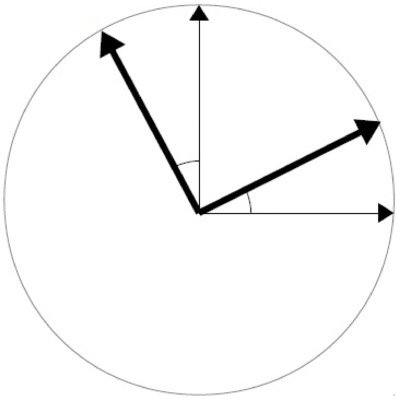
\includegraphics[scale=0.8, page=1]{rydberg_version2_graphics.pdf}
\vspace*{1em}
   \begin{overpic}[
%grid,
width=0.7\columnwidth,
tics=5,
page=1
]{rydberg_version2_graphics}
     \put (97,68) {$\mathbf e_1 e^{i \mathbf e_3 \theta}$}
     \put (15,94) {$\mathbf e_2 e^{i \mathbf e_3 \theta}$}
     \put (47,101) {$\mathbf e_2$}
     \put (100.5,45) {$\mathbf e_1$}
     \put (65,48) {$\theta$}
     \put (45,62) {$\theta$}
  \end{overpic}
\caption{Rotation of $\mathbf{e}_1$ and $\mathbf{e}_2$ about $\mathbf{e}_3$ counterclockwise by an angle $\theta$}
\label{fig:garotation}
\end{figure}

Multiplying Eq.~(\ref{eq:e^itheta}) by $\mathbf e_1$, $\mathbf e_2$, and $\mathbf e_3$, we obtain
\begin{subequations}
\begin{align}
\label{eq:e_1e^itheta}
\mathbf{e}_1e^{ i \mathbf e_3  \theta }&= \mathbf{e}_{1}\cos\theta +\mathbf{e}_2\sin\theta = e^{- i \mathbf e_3  \theta }\mathbf{e}_1, \\
\label{eq:e_2e^itheta}
\mathbf{e}_2e^{ i \mathbf e_3  \theta }&= \mathbf{e}_{2}\cos\theta -\mathbf{e}_1\sin\theta = e^{- i \mathbf e_3  \theta }\mathbf{e}_2, \\
\mathbf{e}_3e^{ i \mathbf e_3  \theta }&= \mathbf{e}_{3}\cos\theta +\mathbf{e}_3  i \mathbf e_3 \sin\theta = e^{ i \mathbf e_3  \theta }\mathbf{e}_3 .
\end{align}
\end{subequations}
%where we used the identities in Eqs.~(\ref{eq:e_1i}) to (\ref{eq:e_3i}). 
 Notice that $\mathbf{e}_1 e^{ i \mathbf e_3  \theta }$ is a rotation of $\mathbf{e}_1$ counterclockwise about $\mathbf{e}_3$ by an angle $\theta$, while  $\mathbf{e}_2 e^{ i \mathbf e_3  \theta }$ is a rotation of $\mathbf{e}_2$ counterclockwise about the same direction and the same angle. Notice, too, that the argument of the exponential changes sign when $\mathbf{e}_1$ or $\mathbf{e}_2$ trades places with the exponential, while $\mathbf{e}_3$ commutes with the exponential.

A vector $\mathbf a$ in 2D can be expressed in both rectangular and polar forms:
\begin{equation}
\label{eq:a is xe_1 + ye_2}
\mathbf a = a_x\mathbf e_1 + a_y\mathbf e_2  = a\mathbf e_1 e^{ i \mathbf e_3 \theta}.
\end{equation}
Expanding the exponential using Eq.~(\ref{eq:e_1e^itheta}) and separating the $\mathbf e_1$ and $\mathbf e_2$ components, we arrive at the standard transformation equations for polar to rectangular coordinates:
\begin{subequations}
\begin{align}
x &= a\cos\theta,\\
y &= a\sin\theta.
\end{align}
\end{subequations}
%The inverse transformations immediately follow:
%\begin{subequations}
%\begin{align}
%a &= x^2 + y^2,\\
%\theta &=\tan^{-1}(y/x).
%\end{align}
%\end{subequations}

We may also factor out $\mathbf e_1$ in Eq.~(\ref{eq:a is xe_1 + ye_2}) either to the left or to the right to get
\begin{subequations}
\begin{align}
\mathbf a &= \mathbf e_1\hat a = \mathbf e_1(x +  i \mathbf e_3  y) = \mathbf e_1 ae^{ i \mathbf e_3 \theta},\\
\mathbf a &= \hat a^*\mathbf e_1 = (x -  i \mathbf e_3  y)\mathbf e_1 = ae^{- i \mathbf e_3 \theta}\mathbf e_1.
\end{align}
\end{subequations}
Factoring out $\mathbf e_1$ yields the definition of the complex number $\hat a$ and that of its complex conjugate $\hat a^*$:
\begin{subequations}
\begin{align}
\hat a &= a_x +  i \mathbf e_3  a_y = ae^{ i \mathbf e_3 \theta},\\
\hat a^* &= a_x -  i \mathbf e_3  a_y = ae^{- i \mathbf e_3 \theta}.
\end{align}
\end{subequations}
In general, we have the following relations:
\begin{subequations}
\begin{align}
\label{eq:e_1a is a*e_1}
\mathbf e_1\hat a &= \hat a^*\mathbf e_1,\\
\label{eq:e_2a is a*e_2}
\mathbf e_2\hat a &= \hat a^*\mathbf e_2,\\
\label{eq:e_3a is ae_3}
\mathbf e_3\hat a &= \hat a\mathbf e_3.
\end{align}
\end{subequations}
That is, $\mathbf e_1$ and $\mathbf e_2$ both changes the complex number $\hat a$ to its conjugate $\hat a^*$ after commutation, while $\mathbf e_3$ simply commutes with $\hat a$ \cite{jancewicz, geomaloptics, vold, hestenesoersted}.


\end{document}